\documentclass{article}
\pagestyle{myheadings}
\usepackage{graphicx}

%------------------------------------------------------------------------------
\newcommand{\stardoccategory}  {Starlink User Note}
\newcommand{\stardocinitials}  {SUN}
\newcommand{\stardocnumber}    {52.5}
\newcommand{\stardocauthors}   {M J Bly}
\newcommand{\stardocdate}      {15 April 1991}
\newcommand{\stardoctitle}     {RGASP --- Reduced GAlaxy Surface Photometry
				package}
%------------------------------------------------------------------------------

\newcommand{\stardocname}{\stardocinitials /\stardocnumber}
\renewcommand{\_}{{\tt\char'137}}     % re-centres the underscore
\markright{\stardocname}
\setlength{\textwidth}{160mm}
\setlength{\textheight}{240mm}
\setlength{\topmargin}{-5mm}
\setlength{\oddsidemargin}{0mm}
\setlength{\evensidemargin}{0mm}
\setlength{\parindent}{0mm}
\setlength{\parskip}{\medskipamount}
\setlength{\unitlength}{1mm}

%------------------------------------------------------------------------------
% Add any \newcommand or \newenvironment commands here
%------------------------------------------------------------------------------

\begin{document}
\thispagestyle{empty}
SCIENCE \& ENGINEERING RESEARCH COUNCIL \hfill \stardocname\\
RUTHERFORD APPLETON LABORATORY\\
{\large\bf Starlink Project\\}
{\large\bf \stardoccategory\ \stardocnumber}
\begin{flushright}
\stardocauthors\\
\stardocdate
\end{flushright}
\vspace{-4mm}
\rule{\textwidth}{0.5mm}
\vspace{5mm}
\begin{center}
{\Large\bf \stardoctitle}
\end{center}
\vspace{5mm}

%------------------------------------------------------------------------------
%  Add this part if you want a table of contents
%  \setlength{\parskip}{0mm}
%  \tableofcontents
%  \setlength{\parskip}{\medskipamount}
%  \markright{\stardocname}
%------------------------------------------------------------------------------

\section{Introduction}

The RGASP package is a reduced version of the Cardiff GASP package, and was
prepared for Starlink bty J Davies. A document: {\it ``The RGASP Reduced GAlaxy
Surface Photometry package}''\/ by Davies gives further details.

\section{Starting RGASP}

The Starlink release of RGASP is contained within a separate top level
directory, and has been assigned the logical name {\tt RGASP\_DIR}. This logical
is defined as {\tt RGASP\$DISK:[RGASP]}. Each site will have set its own
{\tt RGASP\$DISK} logical name.

A symbol {\tt RGASPSTART} has been defined as {\tt @RGASP\_DIR:RGASP} in the
standard Starlink login procedure ({\tt SSC:LOGIN.COM}). When executed,
{\tt RGASPSTART} will set up the RGASP commands as DCL symbols.

To make the RGASP commands available, type:
\begin{verbatim}
      $ RGASPSTART
\end{verbatim}
or include it in your own LOGIN.COM

An example of how an image may be displayed is provided in Appendix A, using
the test data provided with RGASP.

\section{Notes}

\begin{enumerate}
\item RGASP has been modifed to allow the use of IKON and Xwindows displays,
and PostScript printers. Most standard Starlink diplays/printers may be used.

\item The size of the packages has been reduced buy
excluding some of the GASP package facilities.

\item Users should disregard the references to RGASPLOGIN in the document by
Davies above, and use the Starlink provided method of starting RGASP.
\end{enumerate}

\pagebreak
\appendix
\section{Examples}
\subsection{Image Display}

The following example uses the data provided with RGASP to produce an image of
a galaxy on an IKON image display device.

\begin{verbatim}
      $ rgaspstart
       + RGASP commands available
      $ name rgasp_dir:data
      $ dispick

      Number of plots across the screen ?
      1
      Graphics device/type (? to see list): ikon
      Suffix of data-file to be opened? (eg. dat or pix etc.)
      dat
        9999 Frames in the file.  frame  ?
      1

      Whole image ?     (y/n)
      y
      Highest pixel in region is   32042.00
      Lowest pixel in region is  0.0000000E+00

                Scale
      Enter value of highest pixel
      2000
      Enter value of lowest pixel
      500

      Log or linear display ? - type 1 for lin, 2 for log.
      2
      (auto-log)
      Frame            1 done.
      Next job (co,br,dr,mo,fi,fr,re,pl,de,go,ll,sc,ne,po,ti,ex or help) ?
      go

      Frame            1 done.
      Next job (co,br,dr,mo,fi,fr,re,pl,de,go,ll,sc,ne,po,ti,ex or help) ?
      ti
      Title for the plot?   (max - 50 characters)
      RGASP Test (DATA.DAT, high=2000,low=500)
      Next job (co,br,dr,mo,fi,fr,re,pl,de,go,ll,sc,ne,po,ti,ex or help) ?
      ex
      FORTRAN STOP
      $
\end{verbatim}
The image produced looks similar to that shown in Figure \ref{fig:plot}, appended.
{\bf NOTE}{\it The figure page will be blank if the {\tt .DVI} file for this
document was not translated using the DVIPS translator for PostScript
printers.}

\pagebreak
\subsection{Figure 1}

The image included in this document was produced using the following:

\begin{verbatim}
      $ rgaspstart
       + RGASP commands available
      $ name rgasp_dir:data
      $ dispick

      Number of plots across the screen ?
      1
      Graphics device/type (? to see list): pscript_ptex
      Suffix of data-file to be opened? (eg. dat or pix etc.)
      dat
        9999 Frames in the file.  frame  ?
      1

      Whole image ?     (y/n)
      y
      Highest pixel in region is   32042.00
      Lowest pixel in region is  0.0000000E+00

                Scale
      Enter value of highest pixel
      2000
      Enter value of lowest pixel
      500

      Log or linear display ? - type 1 for lin, 2 for log.
      2
      (auto-log)
      Frame            1 done.
      Next job (co,br,dr,mo,fi,fr,re,pl,de,go,ll,sc,ne,po,ti,ex or help) ?
      po
      Next job (co,br,dr,mo,fi,fr,re,pl,de,go,ll,sc,ne,po,ti,ex or help) ?
      go

      Frame            1 done.
      Next job (co,br,dr,mo,fi,fr,re,pl,de,go,ll,sc,ne,po,ti,ex or help) ?
      ti
      Title for the plot?   (max - 50 characters)
      RGASP Test (DATA.DAT, high=2000,low=500)
      Next job (co,br,dr,mo,fi,fr,re,pl,de,go,ll,sc,ne,po,ti,ex or help) ?
      ex
      FORTRAN STOP
      $
\end{verbatim}

\begin{figure}
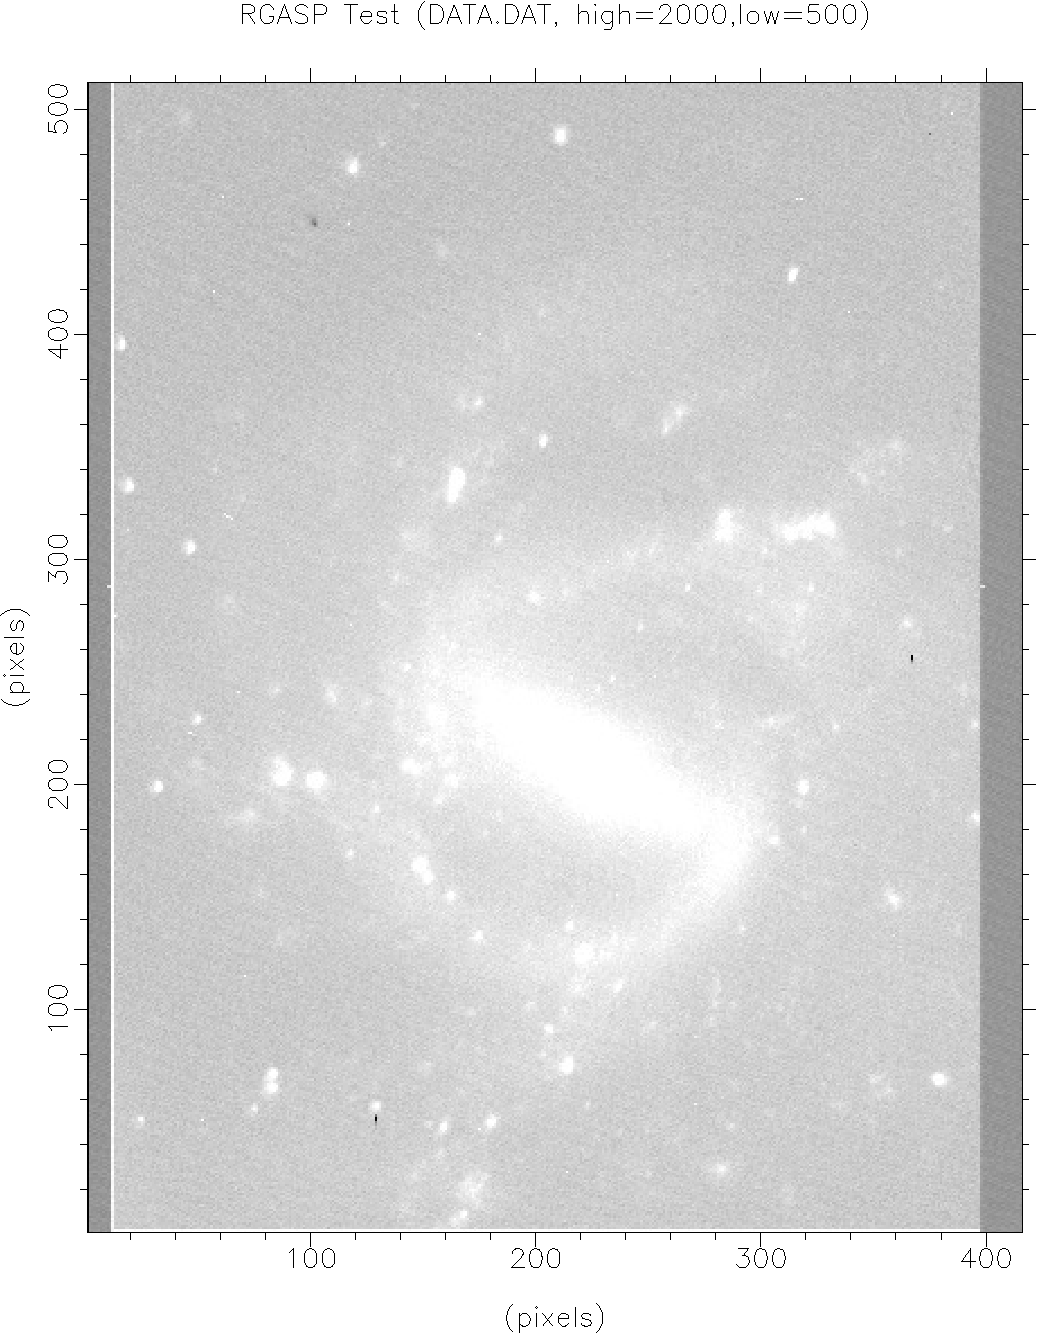
\includegraphics[width=\textwidth]{sun52-figure}
\caption{RGASP Plot using the test data.}
\label{fig:plot}
\end{figure}

\end{document}
